% !TEX root = ../DP_Vik_Tomas_2013.tex
\chapter{Návrh}
Návrh aplikace bude postupovat od shrnutí požadované funkčností přes detailní návrh grafického uživatelského rozhraní po samotný návrh algoritmické části aplikace. V několika následujících sekcích bude tedy přesně vymezen rozsah aplikace a nastíněn způsob jejího řešení.

\section{Návrh funkcionality}
\label{sec:navrh-funkcionality}
Aplikace musí splňovat požadavky dle zadání. Musí umožňovat přidávat, sledovat, prioritizovat a kategorizovat zboží, zobrazovat jeho cenu a její vývoj. Dále bude tato základní funkcionalita detailně popsána a rozšířena o další významné prvky.

V každé sekci bude funkčnost nejprve široce popsána a poté bude tučným písmem napsáno přesné znění výsledné funkcionality.

\subsection{Přihlášení/Odhlášení uživatele}
Přání je z definice vázané na uživatele a je tedy nezbytné uživatele rozlišovat. Standardní způsob jak toto rozlišení provádět ve webových aplikacích je pomocí autentizace a autorizace. Uživatel se nejprve přihlásí pomocí formuláře aplikace. Tím se ověří jeho identita. Poté se mu zobrazují informace určené pouze pro něj. Pokud před přihlášením vytvořil nějaká přání, bude dotázán, jestli chce tato přání uložit do svého seznamu. Uživatel se také může při odchodu ze systému odhlásit.

\textbf{Uživateli bude umožněno se přihlásit do aplikace. Buď pomocí uživatelského jména a hesla, nebo pomocí technologie OAuth. Pokud jako anonymní uživatel vytvořil nějaká přání, bude mu umožněno si je přidat na svůj seznam.}

\textbf{Uživateli bude umožněno se odhlásit z aplikace.}

\subsection{Registrace uživatele}
Pokud se uživatel nebude chtít do aplikace přihlásit pomocí svého OpenID v nějaké z podporovaných autorizačních autorit, bude se muset nejprve do aplikace zaregistrovat. Uživatel vyplní své klíčové údaje:

\begin{itemize}
\item \textbf{E-mail} - jednoznačný identifikátor uživatele v rámci systému
\item \textbf{Uživatelské jméno}
\item \textbf{Heslo}
\end{itemize}

Po potvrzení formuláře bude uživateli vytvořen účet v aplikaci.

\textbf{Uživatel se může zaregistrovat do aplikace pomocí poskytnutí základních údajů.} 

\subsection{Vyhledávání zboží}
\label{sec:vyhledavani}
Toto je klíčová funkcionalita aplikace. V rešerši v předchozí kapitole bylo zjištěno, že vyhledávání zboží je jedna ze základních funkčností aplikací pro srovnávání zboží. Výsledná aplikace tedy bude umožňovat vyhledávání zboží.

\textbf{Uživateli bude umožněno zadat do aplikace vyhledávaný termín jako řetězec a aplikace najde jako výsledek zboží, které v názvu obsahuje tento řetězec. Pokud žádné takové zboží nebude nalezeno, uživateli bude tato informace sdělena.}% a případně mu bude nabídnuto nějaké zboží, které má hledaný termín v popisu.}

\subsection{Přidání a editace přání}
\label{sec:pridani-prani}
Uživateli bude umožněno přidávat zboží do seznamů v podobě takzvaných \emph{přání}. Samotná databáze zboží zůstane odděleně a běžný uživatel\footnote{Jedná se o uživatele, který je klientem aplikace, další druhy uživatelů mohou být administrátor, nebo internetový obchod.} do samotného zboží nebude zasahovat.

Uživateli bude umožněno do seznamu přidat maximálně 20 přání. Omezený počet přání bude usnadňovat uživateli koncentraci a usnadní mu rozhodování\cite{iyengar2004much}. Počet byl daný odhadem a při využívání aplikace bude upraven podle preferencí uživatelů.

Přání bude obsahovat následující základní informace:

\begin{itemize}
\item \textbf{Vazba na zboží} - přání se z definice váže na nějaké zboží. Z tohoto zboží si přání take převezme název.
\item \textbf{Vazba na uživatele} - přání se z definice váže ke konkrétnímu uživateli.
\item \textbf{Obrázek} - obrázek přiřazený k přání pro jeho snazší vizualizaci směrem k uživateli.
\item \textbf{Obchod} - konkrétní obchod, ve kterém si uživatel vybral zboží nakoupit. Používá se pro sledování ceny přání.
\item \textbf{Štítky} - libovolný počet štítků, které uživateli umožňují \textbf{kategorizovat} přání.
\item \textbf{Priorita} - informace o míře priority, tedy jak je přání důležité pro uživatele.
\end{itemize}

Při přidání přání bude uživateli poskytnuta funkce \emph{Rychlá priorita}. Uživatel bude mít při přidání možnost jednoduše rozhodnout jak důležité je pro něj přání, aniž by ho konkrétně musel zařazovat mezi ostatní.

\textbf{Uživateli bude umožněno vytvářet a upravovat přání. Vytvoření bude probíhat pomocí zvolení zboží ve výsledku vyhledávání (viz. kapitola \ref{sec:vyhledavani}). Následně uživatel vyplní informace o přání do vhodného formuláře. Podobný formulář bude sloužit také k editaci přání. Uživateli bude umožněno přidat maximálně 20 přání, po překročení tohoto limitu bude dotázán, jestli chce nově přidaným přáním nahradit nějaké současné přání.}

\subsubsection{Výběr obrázku}
Při vytváření nebo editaci přání je nutné umožnit uživateli vybrat si ze všech obrázků, které jsou v databázi dostupné k danému zboží. Jako první bude uživateli nabídnut nejoblíbenější obrázek.

\subsubsection{Výběr obchodu}
Při vytváření nebo editaci přání je nutné umožnit uživateli vybrat si ze všech obchodů, které jsou v databázi dostupné k danému zboží. Při výběru těchto obchodů musí být uživateli zobrazena aktuální cena zboží v daném obchodu.

\subsection{Mazání přání}
Pokud se uživatel rozhodne, že přání už déle není aktuální, může ho smazat. Smazáním ho odstraní nenávratně ze seznamu svých přání.

\textbf{Uživateli bude umožněno odstranit přání ze svého seznamu.}

\subsection{Splnění přání}
Uživatel může označit přání za splněné. Tímto se přání odstraní ze standardního seznamu a přesune se do seznamu splněných přání, u kterých už se nesleduje cena. Tato přání zůstávají v systému pouze jako informace pro uživatele.

\textbf{Uživateli je umožněno označit přání jako splněné. Tímto označením se přání přesune do seznamu splněných přání.}

\subsection{Změna priority přání}
Jednotlivým přáním je při vytvoření přiřazena uživatelem nadefinovaná, orientační priorita. Tuto prioritu může uživatel měnit. Přání jsou v seznamech řazena podle priority, a tedy po změně priority se změní řazení přání.

\textbf{Uživatel může měnit prioritu přání.}

\subsection{Zobrazení štítků}
\label{sec:zobrazeni-stitku}
Jak bylo napsáno v sekci \ref{sec:pridani-prani}, přání je možné kategorizovat pomocí tzv. štítků. Uživatel musí mít možnost prohlédnout si všechny štítky, které přidal k přáním na jednom místě. Zároveň by u štítků měla být zobrazena informace o tom, kolik přání je daným štítkem označeno. Tato informace může sloužit jako ukazatel důležitosti/četnosti štítku.

\textbf{Uživatel si může zobrazit přehled všech štítků, které přiřadil k jednotlivým přáním.}

\subsection{Zobrazení přehledu přání}
Všechna přání, která uživatel vytvoří, musí být následně uživateli nějakým způsobem zobrazována. Přání mohou být zobrazena buď všechna najednou, nebo mohou být zobrazena pouze přání s konkrétním štítkem. Tento omezený seznam přání se zobrazí pomocí zvolení nějakého štítku ze seznamu štítků (viz. kapitola \ref{sec:zobrazeni-stitku}).

\textbf{Uživatel si může zobrazit přehled buď všech přání, nebo přání obsahujíc konkrétní štítek.}

\subsection{Sledování průběhu cen}
Systém bude schopný u veškerého zboží sledovat cenu v jednotlivých obchodech. Vývoj ceny bude vhodným způsobem zobrazován uživateli u jeho přání. Zároveň bude systém schopný upozornit uživatele na prudké změny ceny jeho přání (primárně snížení cen).

\subsection{Zobrazení nápovědy}
U nepřihlášeného uživatele se očekává nulová zkušenost s aplikací, proto tedy budou důležité ovládací prvky opatřeny nápovědou, která uživateli ujasní jejich princip. Nápověda nemusí být obsáhlá, návrh uživatelského rozhraní se zaměří na jednoduchost používání aplikace i bez nápovědy.

\textbf{Aplikace bude vhodným způsobem zobrazovat nepřihlášenému uživateli nápovědu u klíčových ovládacích prvků.}

\subsection{Automatické doplňování}
V každém textovém poli, kde je aplikace schopna napovědět uživateli pravděpodobný vstup, by mělo fungovat automatické doplňování\footnote{Známé pod svým anglickým názvem: Autocomplete}. Těmito poli jsou v aplikaci vstup pro vyhledávání a vstup s názvy štítků, kterými bude označeno přání.

\textbf{Aplikace bude ve vyhledávání a vkládání štítků podporovat automatické doplňování.}

\subsection{Nezahrnuté funkce z rešerše}
Některé funkce zmíněné v rešerši nebudou v aplikaci z různých důvodů zahrnuty. Tyto funkce zde budou vyčteny a u každé bude uveden důvod jejího vyloučení z funkčních požadavků.

\subsubsection{Mazání bez potvrzování}
V kapitole \ref{sec:astrid} bylo popsáno mazání úkolů ze seznamu. Toto mazání fungovalo tak, že uživatel kliknul na tlačítko smazat a úkol se okamžitě smazal. Uživateli se pouze v horní části stránky zobrazil panel, kde mohl akci vrátit zpět.

Tento způsob mazání je vhodný pro manipulaci s velkým množstvím entit. Ve výsledné aplikaci bude maximální počet 20 přání a od uživatele se neočekává, že by je vytvářel a mazal tak často, aby mazání bez potvrzování přineslo výraznou přidanou hodnotu. Naopak chování aplikace by se odlišovalo od standardu, a to by ve výsledku mohlo snadnosti ovládání aplikace spíše uškodit.

\subsubsection{Řazení podle více kritérií}
V rešerši bylo zmíněno, že mnoho aplikací umožňuje řadit své entity podle vícero kritérií. Logickými kritérii u přání by bylo datum přidání, cena a např. míra změny ceny.

Tato funkcionalita není ve výsledné aplikaci nezbytná, opět se počítá s tím, že přání bude méně než 20. Přání s aktuální výhodnou cenou uvidí uživatel hned po přihlášení a v přehledech mu budou řazena podle priority.

\section{Návrh grafického uživatelského rozhraní}
\label{sec:navrh-gui}
Grafické uživatelské rozhraní (dále GUI) usnadňuje používání aplikace pomocí prezentování informací formou, která je snadná na osvojení a manipulaci s informacemi. Použití vizuálních prvků (přepínačů, tlačítek, posuvníků, atp.) usnadňuje uživateli učení tím, že mu poskytuje intuitivní rozhraní pro práci s aplikací. Špatný návrh GUI může aplikaci uškodit, znepřehlední dodávané informace a neodhalí uživateli všechnu funkcionalitu. Tím uživatele zpravidla donutí k memorování kroků k průchodu běžnými scénáři\cite{toby2001expgui}.

Dobrý design GUI se vyznačuje tím, že po uživateli nevyžaduje žádné memorizování zacházení s aplikací. GUI by přesto mělo umožňovat zrychlený průchod aplikací pomocí zkratek\cite{toby2001expgui}.

Cíle správného návrhu uživatelského rozhraní jsou následující\cite{galitz2007essential}:
\begin{itemize}
\item omezit vizuální práci
\item omezit intelektuální práci
\item omezit množství informací k zapamatování
\item omezit motorickou práci
\item minimalizovat, nebo eliminovat jakékoli problémy nebo instrukce spojené s použitou technologií.
\end{itemize}
Výsledkem takovéhoto návrhu bude vždy lepší produktivita a zvýšená satisfakce uživatele\cite{galitz2007essential}.

Celý návrh je zaměřen na omezení počtu ovládacích prvků a všeobecnou jednoduchost sytému. Ovládací prvky musí mít opodstatněnou svoji funkci.

\subsection{Proces návrhu}
Při návrhu uživatelského rozhraní se nejprve vytvoří seznam operací, které může uživatel v aplikaci provést, tzv. task list. Tyto operace se poté zahrnou do skupin na základě jejich funkce a z takto zpracovaných operací se vytvoří takzvaný task graph, tedy diagram, na kterém bude přesně zobrazeno, kdy k dané operaci může dojít a jaký bude mít následek.

Podle tohoto grafu poté bude vytvořen tzv. wireframe, tedy nakreslené obrazovky aplikace s rozvržením informací a ovládacích prvků.

\subsection{Seznam operací}
Operace se dělí na dva základní druhy, do prvního spadají akce na obrazovkách a přechody mezi obrazovkami, do druhého patří zobrazení obrazovek. Akce které reprezentují zobrazení obrazovek budou v následujícím textu zobrazeny \emph{kurzívou}.
\begin{multicols}{2}
\begin{itemize}
\item \namedlabel{sc-00}{\emph{Základní ovládací prvky}}
\item \namedlabel{op-01}{Návrat na domovskou stránku}%
\item \namedlabel{sc-01}{\emph{Domovská stránka přihlášeného uživatele}}
\item \namedlabel{op-19}{Přechod na stránku s vyhledáváním produktu}%
\item \namedlabel{sc-02}{\emph{Stránka vyhledávání produktu}}
\item \namedlabel{op-02}{Vyhledání produktu}%
\item \namedlabel{sc-03}{\emph{Stránka s výsledky hledání produktu}}
\item \namedlabel{op-03}{Přidání přání}%
\item \namedlabel{sc-11}{\emph{Formulář pro přidání přání}}
\item \namedlabel{op-04}{Výběr obchodu s produktem přání}%
\item \namedlabel{op-05}{Výběr obrázku přání}%
\item \namedlabel{op-06}{Uložení přidaného přání}%
\item \namedlabel{sc-12}{\emph{Dialog pro výběr přání, které bude nahrazeno}}
\item \namedlabel{op-26}{Vybrání přání k nahrazení}
\item \namedlabel{op-27}{Potvrzení dialogu nahrazení přání}
\item \namedlabel{op-21}{Přechod na seznam všech přání}%
\item \namedlabel{sc-04}{\emph{Stránka se seznamem všech přání}}
\item \namedlabel{op-07}{Změna priority přání}%
\item \namedlabel{op-25}{Přechod na detail přání}
\item \namedlabel{sc-05}{\emph{Formulář pro editaci/detail přání}}
\item \namedlabel{op-08}{Označení přání jako splněné}%
\item \namedlabel{op-09}{Smazání přání}%
\item \namedlabel{sc-06}{\emph{Dialog při mazání přání}}
\item \namedlabel{op-11}{Potvrzení dialogu pro mazání přání}%
\item \namedlabel{op-12}{Zamítnutí dialogu pro mazání přání}%
\item \namedlabel{sc-07}{\emph{Komponenta se seznamem štítků}}
\item \namedlabel{op-13}{Výběr štítku}
\item \namedlabel{sc-08}{\emph{Zobrazení seznamu přání označených štítkem}}
\item \namedlabel{op-14}{Přihlášení uživatele pomocí uživ. jména a hesla}%
\item \namedlabel{op-15}{Přihlášení uživatele pomocí Google}%
\item \namedlabel{op-16}{Odhlášení uživatele}%
\item \namedlabel{op-22}{Přechod na dialog registrace}%
\item \namedlabel{sc-09}{\emph{Formulář registrace uživatele}}
\item \namedlabel{op-23}{Potvrzení dialogu registrace uživatele}%
\item \namedlabel{op-24}{Zamítnutí dialogu registrace uživatele}%
\item \namedlabel{sc-10}{\emph{Dialog na přidání přání nepřihlášeného uživatele}}
\item \namedlabel{op-17}{Potvrzení dialogu na přidání přání nepřihlášeného uživatele}%
\item \namedlabel{op-18}{Zamítnutí dialogu na přidání přání nepřihlášeného uživatele}%
%op27--sc12
\end{itemize}
\end{multicols}

\subsection{Analýza operací}
Operace je pro pokračování v návrhu GUI potřebné rozdělit do skupin podle jejich logického uspořádání. Dále je nutné každé operaci přiřadit důležitost (např. chybové zprávy nejdříve). Rozdělení operací na operace zobrazující informace a operace vyžadující uživatelský vstup bylo pro přehlednost provedeno už při jejich výčtu.

\subsubsection{Hlavní akce aplikace}
\label{sec:hlavni-akce}
Tato skupina obsahuje hlavní akce, které uživatel může provádět kdykoli při práci s aplikací.

Tyto akce jsou dostatečně důležité na to, aby byly jejich ovládací prvky umístěné v layoutu stránky\footnote{Layout neboli rozvržení je v moderních webových aplikacích šablona, do které se vkládá obsah stránek. Tato šablona zpravidla obsahuje hlavičku stránky, hlavní ovládací prvky, patičku a poté prostor pro samotný obsah, který je posléze doplněn.}.
\begin{itemize}
\item \textbf{\ref{op-01}} Je naprosto nezbytné, aby se uživatel měl možnost vrátit z jakékoli stránky na výchozí stránku\cite{molich1990improving}. Díky této vlastnosti se uživateli nikdy nestane, že by nevěděl kam na stránce pokračovat, při nejhorším se vždy vrátí na začátek.
\item \textbf{\ref{op-19}} Uživatel musí mít vždy možnost přejít přímo na přidání přání. Největším usnadněním je umístit velké tlačítko na každou stránku.
\item \textbf{\ref{op-13}} Uživatel si třídí svá přání do kategorií pomocí štítků a je důležité, aby je měl stále na očích (to umožňuje \ref{sc-07}) a zároveň se mohl podívat na přání označená daným štítkem.
\item \textbf{\ref{op-21}} Přehled všech přání je další základní funkcionalita, jejíž zpřístupnění musí být uživateli co nejvíce usnadněno.
\end{itemize}
Následující čtyři operace souvisí s přihlášením. Jejich umístěním na každou stránku nejen že umožňujeme uživateli aby se kdykoli přihlásil/odhlásil/zaregistroval, ale zároveň ho tím vždy informujeme o tom, jestli je přihlášený což odpovídá principu zřetelného stavu systému\cite{molich1990improving}.
\begin{multicols}{2}
\begin{itemize}
\item \ref{op-14}\footnote{Přihlášení a registrace jsou umožněny pouze nepřihlášenému uživateli a odhlášení pouze přihlášenému.\label{footnote-login}}
\item \ref{op-15}\footref{footnote-login}
\item \ref{op-16}\footref{footnote-login}
\item \ref{op-22}\footref{footnote-login}
\end{itemize}
\end{multicols}

\subsection{Akce manipulace s přáními}
Další skupinou jsou akce, které nějakým způsobem pracují s přáními.
\begin{multicols}{2}
\begin{itemize}
\item \ref{op-02}
\item \ref{op-03}
\item \ref{op-04}
\item \ref{op-05}
\item \ref{op-06}
\item \ref{op-07}
\item \ref{op-08}
\item \ref{op-09}
\item \ref{op-11}
\item \ref{op-12}
\item \ref{op-17}
\item \ref{op-18}
\end{itemize}
\end{multicols}

Těchto akcí je vzhledem k rázu aplikace naprostá většina. Proto je u nich důležitá priorita.

\subsubsection{Obrazovky}
Zbytek operací je zobrazení obrazovek. Obrazovky se ještě dělí na hlavní obrazovky, které zabírají celou stránku, informativní komponenty, které zabírají pouze část stránky a dialogy, informativní a chybová hlášení, které uživatel může zavřít a zobrazují se zřetelně v popředí stránky.

Jedna speciální obrazovka jsou hlavní ovládací prvky. To jsou ovládací prvky, které umožňují uživateli provádět hlavní akce operace (viz. \ref{sec:hlavni-akce}). Tato obrazovka je přítomná na všech hlavních obrazovkách.

\subsection{Diagram operací}
I ty nejjednodušší webové stránky jsou dynamické. Vztah mezi uživatelem a stránkou je daný uživatelovou interakcí. Uživatelův průchod webovou stránkou musí být naplánován. Diagramy operací jsou nástrojem, jak tento průchod navrhnout a vizualizovat\cite{brown2007communicating}.

Na rozdíl od map stránek\footnote{Site map - diagram prezentující strukturu informací na stránce. Tento hierarchicky zobrazuje jaká stránka patří pod kterou. Nejčastěji jsou stránky v tomto diagramu zobrazovány od shora dolů, kde se nahoře nachází ``rodičovské'' stránky\cite{brown2007communicating}.} kde je vztah stránek vyjádřen hierarchicky (jedna stránka náleží jiné), je u diagramu operací vztah mezi stránkami sekvenční (operace na jedné stránce vede ke stránce druhé)\cite{brown2007communicating}.

Diagramy operací nemají ustálenou notaci\footnote{Několik konvencí bylo zavedeno, ale žádná z nich nebyla akceptována širokou veřejností jako standard\cite{brown2007communicating}.}. V následujícím odstavci je popsána notace diagramu, která je použita v této práci.  

Jedná se o orientovaný graf s dvěma druhy uzlů: obrazovky a akce. Orientované hrany mezi těmito uzly znázorňují jak akce vedou ke zobrazení informací a zároveň z jakých obrazovek je možné vyvolat jaké akce.

Každá hrana v tomto grafu je orientovaná a zároveň musí incidovat s jedním uzlem typu obrazovka a s jedním uzlem typu akce.

Diagram operací ukazuje vztah mezi jednotlivými operacemi, zpravidla je možné všechny operace v grafu i předešlých seznamech rozdělit na detailnější operace.

\begin{figure}[htb]
\begin{center}
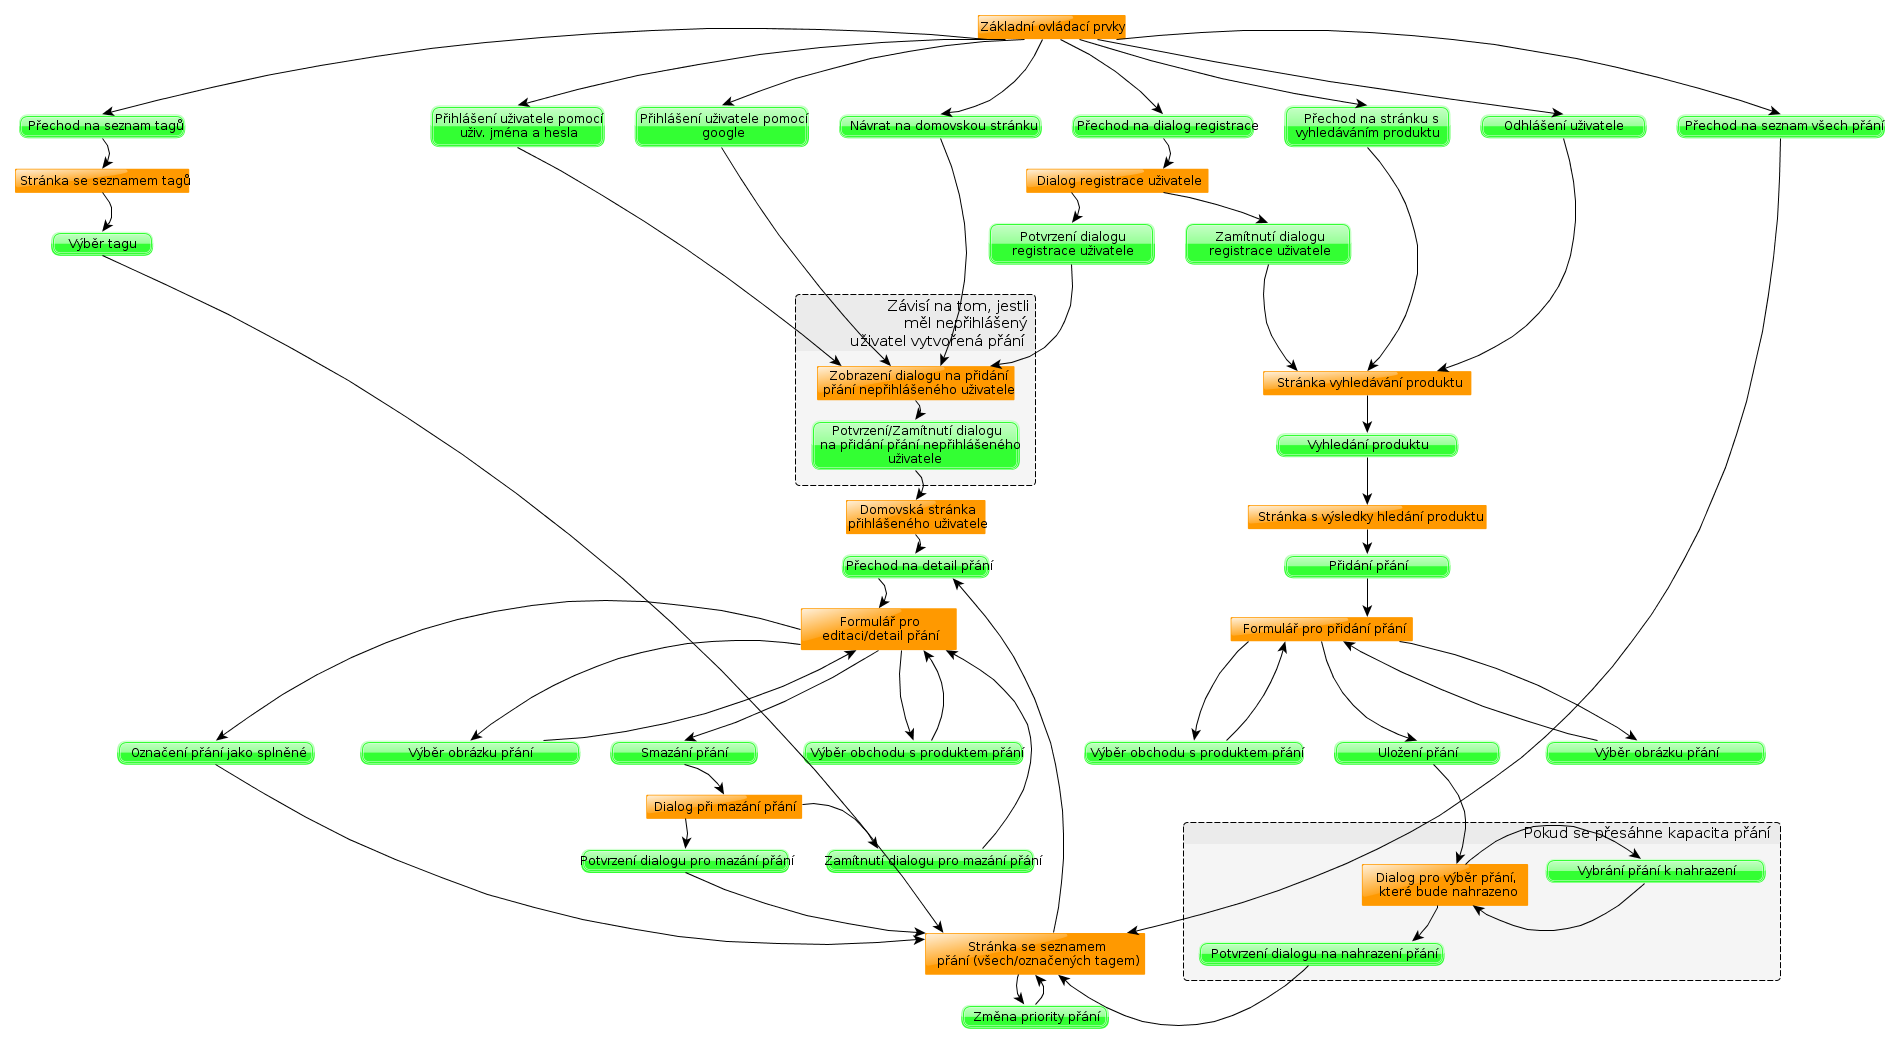
\includegraphics[width=150mm]{./pictures/taskGraph.png}
\caption{Diagram operací pro návrh GUI}
\label{fig:taskGraph}
\end{center}
\end{figure}

\subsection{Wireframe - Drátěný model}
Wireframe je množství ilustrací, které ukazují v malém, nebo velkém detailu obsah každé stránky. Typicky jsou nakresleny pomocí jednoduchých čar, není to vyčerpávající návrh vzhledu. Mimo jiné ukazují, jaké informace budou dostupné na jaké stránce. Wireframe je jedním z více kontroverzních dokumentů návrhu uživatelského rozhraní, protože spojují dohromady (tedy nerozlišují mezi) strukturou informací a jejich vizuálním návrhem. Jinými slovy wireframe překračuje hranici mezi strukturou (jaké mají mezi sebou různé informace vztah) a vzhledem (jak budou informace prezentovány na obrazovce)\cite{brown2007communicating}.

Kompletní návrh je včetně obrázků v příloze \ref{chp:wireframe}. Proto v této části práce budou pouze stručně popsány nejdůležitější body.

\subsubsection{Využití Nielsenovy heuristiky při návrhu}
Při návrhu obrazovek bylo postupováno podle všech pravidel heuristiky pro vyhodnocení uživatelských rozhraní popsané Jakobem Nielsenem\cite{molich1990improving}. Konkrétně:
\begin{enumerate}
\item \textbf{viditelnost stavu systému} - název stránky umístěný v horní části stránky
\item \textbf{shoda systému a reálného světa} - veškeré názvosloví v aplikaci, např. štítky a přání, ovládací prvky na obrazovkách, jsou zobrazeny v logickém pořadí, tedy důležitější nahoře, nebo vlevo
\item \textbf{svobodné akce uživatele} - aplikace vždy umožňuje pomocí zpět přejít na předchozí stránku, odkaz na domovskou stránku je vždy dobře dostupný (dvakrát umístěn v layoutu stránky)
\item \textbf{konzistence a standardy} - hlavní menu je v levém panelu, název stránky odkazuje na hlavní stranu
\item \textbf{prevence chyb} - použití JavaScript validací, které uživatele informují o chybě ještě než ji odešle na server. Minimalizace textových vstupních polí pro uživatele
\item \textbf{preference rozpoznání před vzpomínáním} - všechny důležité informace jsou uživateli zobrazeny na obrazovce se kterou právě pracuje. Např. v obrazovce \ref{sc-10} jsou uživateli všechna přání vyčtena, místo toho aby si musel pamatovat, která přání jako nepřihlášený uživatel vytvořil.
\item \textbf{flexibilita a efektivnost použití} - Nepřihlášenému uživateli se zobrazuje nápověda u hlavních ovládacích prvků, zatímco přihlášenému (tedy zkušenému) nikoli. Systém je celkově velmi jednoduchý, žádné zkratky v něm nebyly navrženy.
\item \textbf{efektivní informační design} - množství zobrazených informací bylo pro přehlednost minimalizováno. U přání se vývoj ceny zobrazuje pomocí grafu.
\item \textbf{pomoc při rozpoznávání, stanovení chyb a následné zotavení} - chybové zprávy byly navrženy s ohledem na toto pravidlo
\item \textbf{nápověda a dokumentace orientovaná na úkoly} - Systém obsahuje pouze minimální nápovědu poskytnutou formou popup oken\footnote{JavaScriptová okénka, která se zobrazí pokud uživatel najede myší nad daný prvek.} nad hlavními ovládacími prvky.
\end{enumerate}

\section{Návrh implementace}
Přestože je implementace výsledné aplikace daná vybranou technologií, existuje několik částí, které jsou spíše algoritmické. Na tyto části nemá použitá technologie velký vliv. Přesně tyto části aplikace budou rozebrány v úvodu této kapitoly.
Ve druhé části bude popsán a zdůvodněn výběr technologií, které budou použity při tvorbě výsledné aplikace.

\subsection{Algoritmus pro vytvoření spojového seznamu v databázi}
Běžný způsob jak uložit data v moderních aplikacích je uchování v relačních databázích. Takovým způsobem budou uložena i jednotlivá přání ve výsledné aplikaci.

Každé přání má prioritu. Tato priorita je navržena jako odkaz na umístění v seznamu všech přání. Např. máme tři přání, jedno má vysokou, druhé střední a třetí nízkou prioritu. Vysoká priorita prvního přání je informace o tom, že přání má být umístěno na prvním místě v seznamu. Střední priorita je informace o tom že se přání nachází v seznamu uprostřed atd.

Reprezentace této informace v databázi může být realizována dvojím způsobem, který zároveň určuje algoritmus pro ukládání/získávání přání.

\subsubsection{Priorita jako celé číslo}
Do tabulky přání je možné vložit jeden sloupec s celočíselným datovým typem nazvaný např. |priorita|. Poté se určí, že vyšší hodnota tohoto sloupce znamená vyšší prioritu.
\begin{table}[htb]
	\begin{center}
	  \begin{tabular}{ | l | c | }
	    \hline
	    NÁZEV & PRIORITA  \\ \hline \hline
	    přání1 & 1  \\ \hline
	    přání2 & 2 \\ \hline
	     &  \\ \hline
	  \end{tabular}
	  \caption{Tabulka v databázi s celočíselnou prioritou}
	  \label{tab:integer-priority}
	\end{center}
\end{table}


Nyní stačí vkládat do tabulky přání a nastavovat hodnotu sloupce |priorita| tak, aby odpovídala chtěnému umístění přání v seznamu. Problém nastane ve chvíli, kdy máme přání1 s prioritou=1, přání2 s prioritou=2 (viz tabulka \ref{tab:integer-priority}) a chceme do databáze přidat přání3, které bude mít vyšší prioritu než přání1 a nižší než přání2. V tuto chvíli nemáme žádnou celočíselnou hodnotu priority, kterou bychom mohli přání3 přidělit, abychom dostali kýžený výsledek. Jedinou možností je změnit prioritu už uložených přání tak, aby vzniklo místo pro přání nové.

V tomto příkladu je úprava přání v databázi triviální, ale při větším počtu přání v databázi může být úprava náročná.

\paragraph{Postup pro získání přání seřazených podle priority z databáze}
Přání z databáze jsou získána pomocí klasického příkazu |SELECT| který řadí přání sestupně podle sloupce priorita.

\lstset{language=SQL, style=custom} 
\begin{lstlisting}
SELECT * FROM PRANI ORDER BY PRIORITA DESC;
\end{lstlisting}

\paragraph{Postup pro vložení přání s kolidující prioritou do databáze}
Jak již bylo řečeno výše, vkládání přání je složité, pokud mezi dvěma přánímí neexistuje volná celočíselná priorita(tzn. že se u těchto přání liší hodnota sloupce |PRIORITA| pouze o 1). Problém řeší inkrementace hodnoty ve sloupci |PRIORITA| u všech přání se stejnou, nebo vyšší prioritou než je priorita právě přidaného přání.

Pokud tedy budeme chtít vložit přání s prioritou 3 a taková priorita už v databázi je, kód bude vypadat následovně:

\begin{lstlisting}
BEGIN TRANSACTION;
UPDATE PRANI SET PRIORITA=PRIORITA+1 WHERE PRIORITA >= 3;
INSERT INTO PRANI ('nazev_prani', 3);
COMMIT;
\end{lstlisting}

Na stejném principu bude probíhat i úprava priority už existujícího přání. Přání v aplikaci budou přiřazena k uživatelům, a proto může být v podmínce u příkazu |UPDATE| ještě identifikátor uživatele. Tím se výrazně zmenší počet upravených přání.

Toto řešení priority se hodí pro aplikace, kde se provádí hodně čtení a méně zápisů do databáze.

\subsubsection{Priorita jako odkaz} 
Do tabulky přání je možné vložit sloupec se stejným datovým typem jaký má primární klíč v této tabulce a nazvat ho např. |NEXT_ID|. Tento sloupec bude odkazovat vždy na přání s nížší prioritou.

Na rozdíl od metody s celočíselnou prioritou zde nenastává při vkládání nového záznamu žádný problém. Pokud chci vložit nové přání3 mezi přání1 a přání2 (počáteční stav v tabulce \ref{tab:pointer-priority}), nastavím u přání1 jako následovníka přání3 a u přání3 nastavím jako následovníka přání2.

\begin{table}[htb]
	\begin{center}
	  \begin{tabular}{ | l | c | r | }
	    \hline
	    ID & NÁZEV & NEXT\_ID  \\ \hline \hline
	    1 & přání1 & 2  \\ \hline
	    2 & přání2 & NULL \\ \hline
	     & &  \\ \hline
	  \end{tabular}
	  \caption{Tabulka v databázi s prioritou jako odkaz}
	  \label{tab:pointer-priority}
	\end{center}
\end{table}

Problém u této metody záznamu přichází ve chvíli, kdy chceme dostat přání z databáze seřazené podle priority.

\paragraph{Postup pro získání přání seřazených podle priority z databáze}
Pokud bychom chtěli řešit získání seřazených přání jedním dotazem, museli bychom mít databázi s podporou takzvaných hierarchických, nebo také rekurzivních dotazů. Tyto dotazy za sebe umějí spojovat záznamy na principu rodič-potomek\cite{website:wiki:hierarchical-queries}.

Takový dotaz vypadá pro PL-SQL\footnote{SQL dialekt databází Oracle} následovně\cite{website:oracle:hierarchical}:
\begin{lstlisting}
SELECT * FROM PRANI CONNECT BY PRIOR ID = NEXT_ID
\end{lstlisting}

\paragraph{Postup pro vložení do databáze}
Vložení přání s největší prioritou je triviální. Vloží se nové přání a jako |NEXT_ID| se mu nastaví identifikátor přání, které mělo doteď nejvyšší prioritu. Nalezení takového přání se provede pomocí příkazu:

\begin{lstlisting}
 SELECT * FROM PRANI
    WHERE ID NOT IN (SELECT NEXT_ID FROM PRANI);
\end{lstlisting}

K vložení každého přání musíme znát klíč obou přání, mezi které nové přání vkládáme. V následujícím skriptu vkládáme přání 3 do tabulky \ref{tab:pointer-priority}

\begin{lstlisting}
BEGIN TRANSACTION;
UPDATE PRANI SET NEXT_ID=3 WHERE ID = 1;
INSERT INTO PRANI (3,'prani3', 2);
COMMIT;
\end{lstlisting}

Výsledek operace je znázorněn v tabulce \ref{tab:pointer-priority-result}.

\begin{table}[htb]
	\begin{center}
	  \begin{tabular}{ | l | c | r | }
	    \hline
	    ID & NÁZEV & NEXT\_ID  \\ \hline \hline
	    1 & přání1 & 3  \\ \hline
	    2 & přání2 & NULL \\ \hline
	    3 & prani3 & 2 \\ \hline
	  \end{tabular}
	  \caption{Výsledek přidání přání 3 mezi přání 1 a 2.}
	  \label{tab:pointer-priority-result}
	\end{center}
\end{table}

Při mazání přání je vždy nutné vrátit ukazatel tak aby se "přeskočilo" smazané přání. Kód pro smazání přání3 z tabulky \ref{tab:pointer-priority-result} vypadá následovně:

\begin{lstlisting}
BEGIN TRANSACTION;
UPDATE PRANI SET NEXT_ID=2 WHERE ID = 1;
DELETE FROM PRANI WHERE ID=3;
COMMIT;
\end{lstlisting}

Při úpravě priority přání se spojí kroky smazání a vytvoření přání.

Toto řešení se hodí pro aplikace, kde se více zapisuje a méně čte do databáze.

\subsection{Algoritmus určení počáteční priority přání}
V předchozí sekci (\ref{sec:pridani-prani}) bylo zmíněno, že uživateli bude usnadněno přidání přání pomocí tzv. \emph{Rychlé priority}. V příloze v návrhu drátěného modelu \ref{sec:wireframe-pridani-prani} byl navržen ovládací prvek s třemi tlačítky určujícími prioritu \emph{Nízká}, \emph{Střední} a \emph{Vysoká}. Ve zbytku této kapitoly bude popsán algoritmus, který převede tuto volbu na finální prioritu, která přání zařadí na konkrétní místo do seznamu všech přání.

\subsubsection{Výpočet váhy štítku}
Kromě samotné volby rychlé priority uživatel poskytuje ještě jednu informaci o důležitosti přání, a tou jsou štítky. Algoritmus předpokládá, že často se vyskytující štítky jsou důležitější, než ty s menším výskytem. S tímto předpokladem se dále pracuje.

Normalizovanou váhou štítku rozumíme reálné číslo v intervalu $<0;1>$. Kde 0 je pro štítek, který není přiřazen k žádnému přání a 1 je pro štítek, který je u každého přání. Výpočet váhy je vznikne jednoduchým podílem
\begin{equation}
W = \left\{
  \begin{array}{l l}
    0 & \quad \text{pokud }N_s = 0\\
    \frac{N_s}{N_{all}} & \quad \text{jinak}
  \end{array} \right.
\label{eq:vaha-stitku}
\end{equation}
kde $W$ je váha štítku, $N_s$ je počet přání označených štítkem a $N_{all}$ je počet přání.

\subsubsection{Přiřazení číselných koeficientů rychlé prioritě}
Jak již bylo řečeno uživatel může volit ze tří možností priority: \emph{Nízká}, \emph{Střední} a \emph{Vysoká}. Těmto volbám jsou pro výpočet přiřazeny reálné koeficienty v tabulce \ref{tab:rychla-priorita}.

\begin{table}[htb]
\begin{center}
\begin{tabular}{|l|r|}
\hline
Nízká & 0\\ \hline
Střední & 0,5\\ \hline
Vysoká & 1 \\
\hline
\end{tabular}
\caption{Přiřazení reálných koeficientů k uživatelským volbám.}
\label{tab:rychla-priorita}
\end{center}
\end{table}

\subsubsection{Algoritmus}
Algoritmus využívá všech dříve zmíněných koeficientů. Koeficient váhy štítku je započítán do váženého průměru s váhou 1, zatímco koeficient rychlé priority s váhou pět. Váha štítku se tedy podílí pouze pětinovým podílem na výsledném koeficientu. Algoritmus získá konkrétní přání, pod které do seznamu patří nové přání.
\lstset{language = c, style=custom}
\begin{lstlisting}
/*na zacatku jsou k dispozici tyto promenne
  tags - pole vsech stitku kterymi bylo prani oznaceno
  fast_priority - uzviatelem zvolena rychla priorita
  wishes - pole se vsemi pranimi*/
tag_weight = 0;
//nascitaji se vahy vsech stitku
foreach tag from tags{
	tag_weight += normilezed_weight(tag)
}
//aritmeticky zprumerovana vaha stitku
if(tags.size != 0){
	tag_weight = tag_weight / tags.size
}
//vazeny prumer z vahy stitku a rychle priority
coefficient = 1 - (5*fast_priority + tag_weight) / 6
max_wishes_index = wishes.size - 1
index = round_down(max_wishes_index * coefficient)
above_wish = wishes[index]
\end{lstlisting}

\section{Vybrané technologie}
Na konci návrhu jsou vybrány technologie, které budou použity pro implementaci výsledné aplikace. Některý výběr byl daný také zadáním práce. Primárním cílem je vybrat moderní technologie, které jsou zároveň delší dobu na trhu\footnote{Nevýhodou cutting-edge technologií je i přes jejich zajímavost velké riziko že nebudou podporovány na straně klienta, nebo přestanou být udržovány.}. Zároveň je při výběru zohledněno množství přispěvatelů/příspěvků do kódu aplikace.
\subsection{Programovací jazyk}
Výsledná aplikace bude naprogramována v jazyce \textbf{Ruby}. Toto je část daná zadáním, přesto by byl výběr takový, i kdyby bylo možné vybrat Javu. Důvody pro toto rozhodnutí jsou následující:
\begin{itemize}
\item Dynamicky typované proměnné - názory, zda je tato vlastnost výhoda nebo nevýhoda se liší a každý názor má svá pro a proti. Dynamicky typované proměnné obecně znamenají méně napsaného kódu, tím pádem čitelnější a přehlednější kód. To že není možné některé chyby typu špatné přiřazení apod. rozeznat při kompilaci je potřeba vykompenzovat správnými Unit Testy\footnote{Pod pojem unit testing se zahrnují nástroje, metodika a činnost, jejímž cílem je ověřování správné funkčnosti dílčích částí neboli jednotek zdrojového kódu.}, které by ovšem měla obsahovat aplikace psaná v jakémkoli jazyce\cite{website:oreilly:unit-testing}.
\item Moderní konstrukty jazyka - Ruby poskytuje konstrukty jako bloky a lambda funkce, které programátorovi usnadňují práci.

\end{itemize}

Ruby je výkonově výrazně horší než Java\cite{website:java-ruby-performance}. Např. Twitter původně postavený na Ruby on Rails začal od Ruby ustupovat a nahrazovat ho Javou\cite{website:twitter-ruby-java}. Pro výslednou aplikaci toto není problém, neboť její zátěž nebude vysoká.

\subsection{Framework pro vývoj webové aplikace}
Výsledná aplikace bude postavená na frameworku \textbf{Ruby on Rails} verze 3. Jedná se o framework s nejstarší tradicí. Dále budou popsány všechny faktory, které vedly k jeho výběru:

\begin{itemize}
\item Nejlepší dokumentace - framework je nejstarší na trhu tomu také odpovídá rozsah dokumentace. Framework má vlastní dokumentaci, mnoho psaných publikací, videotutorialů a nespočet krátkých článků online\cite{website:ruby-toolbox-web}\cite{website:ruby-rails-documentation}.
\item Největší počet uživatelů - celkem 23 milionů stáhnutí knihovny, více jak 18 tisíc uživatelů sledující vývoj zdrojových kódů na Github.com. Druhá Sinatra má 7 milionů stáhnutí a méně než 5 tisíc uživatelů sledujících vývoj na Github.com\cite{website:ruby-toolbox-web}.
\item Konvence namísto konfigurace\footnote{Convention over configuration} - Toto je základní myšlenka frameworku. Vše je po vytvoření aplikace základně nakonfigurováno a uživatel mění jen ta nastavení, která potřebuje. To v zásadě znamená, že vývojář píše převážně byznys logiku, zatímco ostatní věci už jsou za něj vyřešeny.
\item Nejvíce přispěvovatelů a příspěvků do zdrojového kódu - stejně jako má Ruby on Rails obrovskou uživatelskou základnu, má také nejvíce vývojářů\cite{website:ruby-toolbox-web}.
\end{itemize}

Výsledná aplikace je více komplexní, proto se pro ni nehodí ve všech ohledech druhý framework Sinatra, jehož hlavní výhodou je jednoduchost \cite{harris2011sinatra}

\subsection{Frontend framework}
Jako HTML, CSS a JavaScript framework bude použit \textbf{Twitter Bootstrap}. Důvody pro jeho použití jsou velice podobné důvodům pro použití frameworku Ruby on Rails a jsou shrnuty dále:
\begin{itemize}
\item Široká uživatelská základna - framework je vůbec nejoblíbenějším projektem na Github.com \cite{website:github-popular}. Existuje velké množství článků o frameworku online. Hodně dalších vytvořených komponent, které je možné rovnou použít.
\item Předpřipravené komponenty - na svých stránkách má framework detailně zpracovanou dokumentaci nejen základních vlastností HTML, které upravuje, ale zároveň i komponent, které jsou tímto framewokrem předpřipraveny.
\item Plugin do Ruby on Rails - je vytvořena knihovna, která snadno integruje framework do Rails\cite{website:github-bootstrap-saas}.
\item Nejvíce přispěvovatelů a příspěvků do zdrojového kódu - do frameworku přispívá takřka 200 vývojářů.
\end{itemize}

\subsection{Metoda napojení na systém srovnávání cen}
Z výše zmíněných metod bude ve výsledné aplikaci použita metoda \textbf{Web Scraping}. Přestože není ideální, byla vybrána z následujících důvodů:
\begin{itemize}
\item Jednoduché nasazení - není třeba žádné vyjednání přístupu se systémy srovnávání cen, žádná autorizace a autentizace.
\item Jednoduchá dokumentace - jak bylo popsáno v kapitole \ref{sec:webscraping}, při vytváření aplikace pro získávání dat vývojář pracuje přímo se stránkou určenou pro koncového uživatele, na které jsou většinou informace jasně a logicky utříděné.
\item Jednoduchá implementace.
\end{itemize}
Nevýhody této metody jsou popsány v kapitole \ref{sec:webscraping}.
